\documentclass[12pt]{book}
\usepackage{tikz}
\usepackage{hyperref}
\hypersetup{
    colorlinks=true, %set true if you want colored links
    linktoc=all,     %set to all if you want both sections and subsections linked
    linkcolor=black,  %choose some color if you want links to stand out
}
\usepackage{amsmath, amssymb}

\usepackage{epigraph}


\renewcommand\epigraphflush{flushright}
\renewcommand\epigraphsize{\normalsize}
\setlength\epigraphwidth{0.7\textwidth}

\definecolor{titlepagecolor}{cmyk}{1,.60,0,.40}

\DeclareFixedFont{\titlefont}{T1}{ppl}{b}{it}{0.5in}


\newcommand\titlepagedecoration{%
\begin{tikzpicture}[remember picture,overlay,shorten >= -10pt]

\coordinate (aux1) at ([yshift=-15pt]current page.north east);
\coordinate (aux2) at ([yshift=-410pt]current page.north east);
\coordinate (aux3) at ([xshift=-4.5cm]current page.north east);
\coordinate (aux4) at ([yshift=-150pt]current page.north east);

\begin{scope}[titlepagecolor!40,line width=12pt,rounded corners=12pt]
\draw
  (aux1) -- coordinate (a)
  ++(225:5) --
  ++(-45:5.1) coordinate (b);
\draw[shorten <= -10pt]
  (aux3) --
  (a) --
  (aux1);
\draw[opacity=0.6,titlepagecolor,shorten <= -10pt]
  (b) --
  ++(225:2.2) --
  ++(-45:2.2);
\end{scope}
\draw[titlepagecolor,line width=8pt,rounded corners=8pt,shorten <= -10pt]
  (aux4) --
  ++(225:0.8) --
  ++(-45:0.8);
\begin{scope}[titlepagecolor!70,line width=6pt,rounded corners=8pt]
\draw[shorten <= -10pt]
  (aux2) --
  ++(225:3) coordinate[pos=0.45] (c) --
  ++(-45:3.1);
\draw
  (aux2) --
  (c) --
  ++(135:2.5) --
  ++(45:2.5) --
  ++(-45:2.5) coordinate[pos=0.3] (d);   
\draw 
  (d) -- +(45:1);
\end{scope}
\end{tikzpicture}%
}


\usepackage{xepersian}
\settextfont[Scale=1]{Vazir}
\usepackage{tikz-network}
\usetikzlibrary{positioning}
\usetikzlibrary{patterns}

\renewcommand{\baselinestretch}{1.3} 

\begin{document}

%\title{آمار و احتمالات مهندسی}
%\maketitle


\begin{titlepage}
%\noindent
\titlefont 
\begin{tikzpicture}
\begin{scope}
\node[scale=3] (b) at (0,0) {احتمالات و آمار};
\node[scale=3] (b) at (0,-2) {مهندسی};
\end{scope}
\end{tikzpicture}


\null\vfill
\vspace*{1cm}
\noindent
\hfill

\titlepagedecoration
\end{titlepage}


\tableofcontents

\chapter{اصول شمارش}

\section{اصول شمارش}

\begin{itemize}
	\item اصل جمع
	\item اصل ضرب
	\item جایگشت
	\item ترتیب
	\item ترکیب
\end{itemize}


\subsection{اصل جمع}
فرض کنید یک کار را بتوان با 2 عمل A یا B انجام داد . اگر عمل A به $n_{1}$ روش و عمل B به $n_{2}$ انجام پذیر باشند و این دو عمل نتوانند همزمان اتفاق بیفتند در این صورت، این کار به $n_{1} + n_{2}$ روش انجام پذیر است .

\begin{align*}
A &\to n_{1}   \\
& & &\Rightarrow & & n_{1} + n_{2} \\
B &\to n_{2}   \\
\end{align*}


برای مثال برای رفتن از نکا به ساری در صورتی که به وسیله ی 

\begin{itemize}
	\item دوچرخه $\leftarrow$ 3 روش
	\item ماشین $\leftarrow$ 2 روش
	\item پیاده $\leftarrow$ 4 روش
\end{itemize}

\begin{tikzpicture}
\Vertex[x=0,size=1,fontscale=1,label=نکا]{A}
\Vertex[x=4,size=1,fontscale=1,label=ساری]{B}
\end{tikzpicture}

مجموعاً به (3+2+4) روش می توان از نکا به ساری رفت، این اعمال از هم مستقل اند .


\subsubsection{مثال}

4 نفر در مکانی با هم برخورد می کنند، اگر هر فرد بخواهد با افراد دیگر دست بدهد، به چند طریق این دست دادن امکان پذیر است ؟

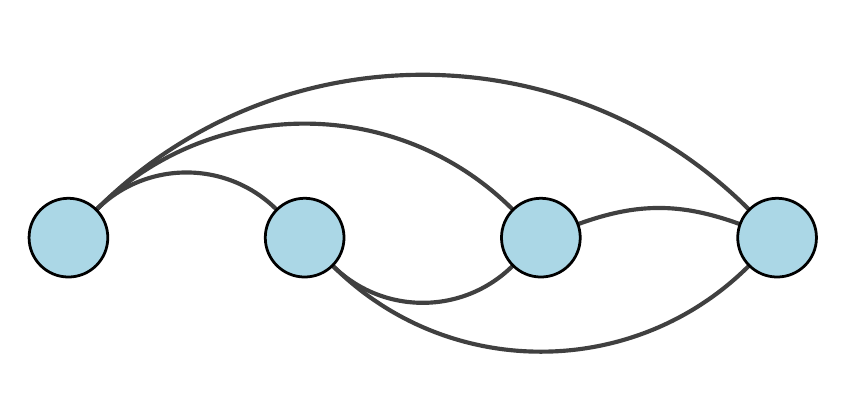
\begin{tikzpicture}
\Vertex[x=0,size=1,fontscale=2]{A} 
\Vertex[x=3,size=1,fontscale=2]{B}
\Vertex[x=6,size=1,fontscale=2]{C}
\Vertex[x=9,size=1,fontscale=2]{D}

\Edge[bend=45](A)(B)
\Edge[bend=45](A)(C)
\Edge[bend=45](A)(D)

\Edge[bend=-45](B)(C)
\Edge[bend=-45](B)(D)
%\Edge[bend=0,lw=3pt](B)(C)

\Edge[bend=20](C)(D)

\end{tikzpicture}


جواب : 
$$
3 + 2 + 1 = 6
$$


\subsection{اصل ضرب}

اگر انجام یک کار شامل 2 مرحله باشد به طوریکه مرحله ی اول به $n_{1}$ روش و مرحله ی دوم برای هر یک از $n_{1}$ روش اول به $n_{2}$ روش انجام پذیر باشد، در این صورت کل کار به $n_{1} * n_{2}$ روش انجام پذیر است .

\subsubsection{مثال}
فرض کنید می خواهیم از نکا به ساری حرکت کنیم، برای انجام این کار دو مرحله وجود دارد .
\begin{itemize}
	\item مرحله ی اول از نکا به سورک به 3 روش
	\item مرحله ی دوم از سورک به ساری به 4 روش
\end{itemize}


در این صورت تمام مسیرهای ممکن برابر است با :\newline

\begin{tikzpicture}
\Vertex[x=0,label=نکا,size=2,fontscale=2]{A} 
\Vertex[x=4,label=سورک,size=2,fontscale=2]{B}
\Vertex[x=8,label=ساری,size=2,fontscale=2]{C}

\Edge[bend=25](A)(B)
\Edge[bend=0](A)(B)
\Edge[bend=-25](A)(B)

\Edge[bend=30](B)(C)
\Edge[bend=10](B)(C)
%\Edge[bend=0,lw=3pt](B)(C)
\Edge[bend=-10](B)(C)
\Edge[bend=-30](B)(C)
\end{tikzpicture}


$$
3 * 4 = 12
$$


\subsubsection{مثال}
گروهی شامل 5 دبیر و 8 مهندس در نظر بگیرید، به چند طریق می توان 2 نماینده شامل 1 دبیر و 1 مهندس از این گروه انتخاب کرد ؟

روش اول : 

$$
\binom{5}{1}  \binom{8}{1}  = 5 * 8 = 40
$$

روش دوم :

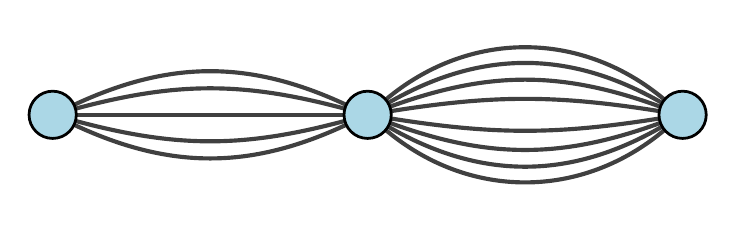
\begin{tikzpicture}
\Vertex[x=0]{A} 
\Vertex[x=4]{B}
\Vertex[x=8]{C}

\Edge[bend=25](A)(B)
\Edge[bend=15](A)(B)
\Edge[bend=0](A)(B)
\Edge[bend=-15](A)(B)
\Edge[bend=-25](A)(B)

\Edge[bend=40](B)(C)
\Edge[bend=30](B)(C)
\Edge[bend=20](B)(C)
\Edge[bend=9](B)(C)
%\Edge[bend=0,lw=3pt](B)(C)
\Edge[bend=-9](B)(C)
\Edge[bend=-20](B)(C)
\Edge[bend=-30](B)(C)
\Edge[bend=-40](B)(C)
\end{tikzpicture}

$$
5 * 8 = 40
$$



\subsubsection{سوال مهم}
با استفاده از مجموعه ی 
$\{ 0, 1, 2, 3, 4 \}$
چند عدد سه رقمی می توان نوشت که 
\begin{itemize}
	\item تکرار ارقام مجاز باشد
	\item تکرار مجاز نباشد
	\item تکرار مجاز و عدد زوج باشد
	\item تکرار مجاز نباشد و عدد فرد باشد
\end{itemize}


جواب :
\begin{LTR}
\begin{itemize}
	\item $4 * 5 * 5 = 100$
	\item $4 * 4 * 3 = 48$
	\item $4 * 5 * 3 = 60$
	\item $3 * 3 * 2 = 18$
\end{itemize}
\end{LTR}



\subsubsection{مثال}
اگر پلاک اتوموبیل ها از 5 شماره ی غیر صفر و یک حرف الفبای فارسی تشکیل شود، تعداد اتوموبیل هایی که می توان شماره کرد را تعیین کنید ؟

$$
\underbrace{9 * 9 * 9 * 9 * 9}_{5 \:\: non-zero \:\: number} * \underbrace{32}_{persian \:\: alphabet} = 9^{5} * 32
$$


\subsection{جایگشت}

اگر n شی متمایز داشته باشیم، می توانیم این اشیا را به فرم های مختلف کنار یکدیگر قرار دهیم. هر آرایش قرار گرفتن این اشیا را یک جایگشت می نامیم. در این صورت تعداد جایگشت ها می شود :
$$
n! = n * (n-1) * (n-2) * \dots * 2 * 1
$$


\subsubsection{مثال}
چند ترتیب مختلف برای معرفی اعضای یک تیم بسکتبال 5 نفره وجود دارد ؟

$$
5! = 5 * 4 * 3 * 2 * 1 = 120
$$


\subsubsection{نکته}
اگر بخواهیم n شی متمایز طوری کنار یکدیگر قرار گیرند که r شی از آنها در کنار هم باشند، در این صورت تعداد جایگشت های ممکن از رابطه ی زیر به دست می آید .

$$
(n-r+1)! r!
$$


\subsubsection{مثال}
به چند طریق ممکن
\begin{itemize}
	\item 2 دانشجوی حسابداری
	\item 5 دانشجوی ریاضی
	\item 3 دانشجوی فیزیک
\end{itemize}
می توانند کنار یکدیگر در یک صف قرار گیرند به طوریکه 5 دانشجوی ریاضی کنار هم باشند ؟

$$
(10-5+1)! 5!
$$


\subsubsection{نکته}
اگر k دسته عنصر داشته باشیم به طوریکه در دسته ی اول $n_{1}$ عضو، در دسته ی دوم $n_{2}$ عضو تا در دسته ی k ام $n_{k}$ عضو داشته باشیم در این صورت تعداد جایگشت های مختلف از رابطه ی زیر محاسبه می شود :\newline

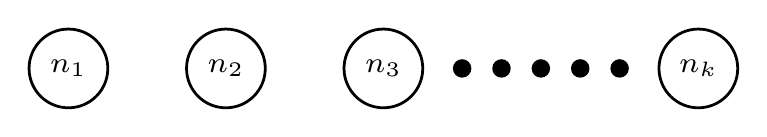
\begin{tikzpicture}
\Vertex[x=0,size=1,color=white,fontscale=1.5,label=$n_{1}$]{A}
\Vertex[x=2,size=1,color=white,fontscale=1.5,label=$n_{2}$]{A}
\Vertex[x=4,size=1,color=white,fontscale=1.5,label=$n_{3}$]{A}
\Vertex[x=5,size=.05,color=black]{A}
\Vertex[x=5.5,size=.05,color=black]{A}
\Vertex[x=6,size=.05,color=black]{A}
\Vertex[x=6.5,size=.05,color=black]{A}
\Vertex[x=7,size=.05,color=black]{A}
\Vertex[x=8,size=1,color=white,fontscale=1.5,label=$n_{k}$]{A}
\end{tikzpicture}

$$
( \: n_{1}! \: n_{2}! \: n_{3}! \: \dots \: n_{k}! \: ) \: k !
$$


\subsubsection{مثال}
به چند طریق 
\begin{itemize}
	\item 4 ایتالیایی
	\item 5 فرانسوی
	\item 2 انگلیسی
\end{itemize}

می توانند در یک ردیف کنار هم قرار گیرند به طوریکه افراد هم ملیت کنار هم باشند .

$$
[ \: 4! \: 5! \: 2! \: ] \: 3!
$$



\subsection{جایگشت دوری(دایره ای)}
تعداد جایگشت های دوری n شی متمایز برابر است با 
$$
(n-1)!
$$


\subsubsection{مثال}
به چند طریق 5 نفر می توانند دور یک میزگرد بنشینند ؟

جواب :
$$
(5-1)!
$$



\subsubsection{نکته}

تعداد جایگشت های n شی متمایز دایره ای که هیچ دو شی دارای همسایه مشترک نباشد 
$$
\frac{(n-1)!}{2}
$$

* هر شخصی در جایگشت دوری همیشه با هر نفر 2 بار همسایه می شود که ما می خواهیم یک بار را حذف کنیم، پس جواب را تقسیم بر 2 می کنیم .

\subsubsection{نکته}
تعداد حالت هایی که بتوان 2 گروه m و n تایی را به صورت یک در میان در یک صف قرارداد به صورت زیر است :

حالت اول ) 
$$
if( m == n ) \to 2!m!n!
$$

حالت دوم )
$$
if( m \neq n ) \to m!n!
$$


\subsubsection{مثال}
به چند طریق 3 زوج می توانند در یک ردیف قرار گیرند هرگاه
\begin{itemize}
	\item 3 خانم کنار هم قرار گیرند
	\item خانم ها و آقایان به طور متناوب ( یکی در میان )
\end{itemize}

جواب :
\begin{itemize}
	\item $( 6-3+1 ) ! 3 ! = 4 ! 3 !$
	\item $[ 3 ! 3 ! ] 2 !$
\end{itemize}


\subsubsection{مثال}
به چند طریق می توان 4 خانم و 4 آقا دور یک میز قرار گیرند به طوری که آقایان کنار هم و خانم ها کنار هم باشند ؟

جواب :

$$
(4-1)!(4-1)!2!
$$



\subsection{ترتیب}
هرگاه بخواهیم r شی از بین n شی متمایز انتخاب کنیم و در یک صف ( اولویت مهم است ) کنار هم قرار دهیم، در این صورت تعداد حالت ها برابر است با :
\begin{itemize}
	\item تکرار مجاز نباشد :
	$$
	\frac{n!}{(n-r)!}
	$$
	\item تکرار مجاز باشد :
	$$
	n^{r}
	$$
\end{itemize}



\subsubsection{مثال}
با حروف کلمه ی History چند کلمه ی 4 حرفی می توان نوشت ؟
\begin{itemize}
	\item تکرار مجاز باشد
	\item تکرار مجاز نباشد
\end{itemize}


\begin{itemize}
	\item 
	$$
	7 * 7 * 7 * 7 = 7^{4}
	$$
	\item 
	$$
	7 * 6 * 5 * 4 = \frac{7!}{3!}
	$$
\end{itemize}




\subsubsection{مثال}
با حروف کلمه ی `فردوسی` چند کلمه ی 3 حرفی بدون تکرار می توان نوشت، به طوریکه حرف اول آن نقطه دار باشد ؟

$$
2 * 5 * 4 = 40
$$


\subsubsection{مثال}
15 نفر در یک مسابقه دوچرخه سواری شرکت می کنند، به چند طریق می توان جوایز اول، دوم، سوم را به افراد شرکت کننده اعطا نمود ؟ (ترتیب / بدون تکرار چون انسان ها تکرار نمی شوند)
$$
P^{15}_{3} = \frac{15!}{(15-3)!} = \frac{15!}{12!}
$$

\subsection{ترکیب}

مفهوم ترکیب : هرگاه بخواهیم r شی از بین n شی متمایز انتخاب کنیم که اولویت انتخاب مهم نباشد 

\subsubsection{اگر تکرار عناصر مجاز نباشد}
تعداد راه های انتخاب برابر است با :
$$
\binom{n}{r} = \frac{n!}{(n-r)!r!}
$$



\subsubsection{اگر تکرار عناصر مجاز باشد}
در این صورت تعداد راه های انتخاب از رابطه ی زیر به دست می آید :
$$
\frac{(n+r-1)!}{(n-1)!r!}
$$


\subsubsection{مثال}
یک گروه شامل 6 مهندس و 10 دبیر می باشد، به چند طریق می توان یک کمیته ی 3 نفره انتخاب کرد ؟
( در کمیته و در تشکیل شورا اولویت مهم نیست و بدون تکرار است چون انسان تکرار نمی شود )

\begin{itemize}
	\item کمیته شامل 3 دبیر باشد
	$$
	\binom{10}{3}
	$$
	\item کمیته شامل 2 دبیر و 1 مهندس باشد
	$$
	\binom{10}{2} \binom{6}{1}
	$$
	\item کمیته شامل حداقل 1 دبیر باشد
	$$
	\binom{10}{1} \binom{6}{2} + \binom{10}{2} \binom{6}{1} + \binom{10}{3}
	$$
	\item حداکثر 1 دبیر
	$$
	\binom{6}{3} + \binom{10}{1} \binom{6}{2}
	$$
\end{itemize}


\subsubsection{مثال}
شخصی 13 نفر را برای شام دعوت می کند، 8 نفر از آنها دور یک میز و بقیه ( 5 نفر ) ، دور میز دیگری می نشینند ، به چند طریق این کار انجام پذیر است ؟
$$
\binom{13}{8} (8-1)! (5-1)!
$$

$\leftarrow \binom{13}{8}  $ تعداد حالت های تقسیم گروه 13 نفره به 2 گروه 8 و 5 نفره

$\leftarrow (8-1)! $ تعداد حالت های نشستن 8 نفر دور یک میز

$\leftarrow (5-1)!$  تعداد حالت های نشستن 5 نفر دور یک میز



\subsubsection{مثال}
با 10 نقطه که نصف آنها روی یک خط واقع هستند چند مثلث می توان ساخت ؟\newline\newline

%\setlength{\unitlength}{1cm}
%\begin{picture}(1,3)
%\put(0,0){\line(1,0){6}}
%\put(0,0){\circle*{1}}
%\put(1,0){\circle*{1}}
%\put(2,0){\circle*{1}}
%\put(3,0){\circle*{1}}
%\put(4,0){\circle*{1}}
%\put(1.8,2){\circle*{1}}
%\put(2.5,1.3){\circle*{1}}
%\put(1.1,2.2){\circle*{1}}
%\put(3.5,1.7){\circle*{1}}
%\put(1.5,1){\circle*{1}}
%\end{picture}

\begin{tikzpicture}
\draw (0,0) -- (10,0) ;
\filldraw[color=black] (1,0) circle (.1cm);
\filldraw[color=black] (3,0) circle (.1cm);
\filldraw[color=black] (5,0) circle (.1cm);
\filldraw[color=black] (8,0) circle (.1cm);
\filldraw[color=black] (9,0) circle (.1cm);
\filldraw[color=black] (2.4,4.1) circle (.1cm);
\filldraw[color=black] (4.6,2.4) circle (.1cm);
\filldraw[color=black] (6.3,4.9) circle (.1cm);
\filldraw[color=black] (7.2,2.5) circle (.1cm);
\filldraw[color=black] (8.5,3.4) circle (.1cm);
\end{tikzpicture}


$$
\binom{5}{2} \binom{5}{1} + \binom{5}{2} \binom{5}{1} + \binom{5}{3}
$$


\chapter{احتمال}

\section{احتمال}

\subsection{تعریف آزمایش تصادفی}

هر آزمایشی که نتیجه ی آن از قبل معلوم نباشد، اما مجموع نتایج آن مشخص باشد ( مثل : پرتاب سکه، پرتاب تاس )

\subsection{تعریف فضای نمونه}
مجموعه ی همه ی نتایج یک آزمایش تصادفی را فضای نمونه می نامیم

برای مثال فضای نمونه برای پرتاب تاس برابر است با :

$$
S = \{ 1 , 2 , 3 , 4 , 5 , 6 \}
$$

\subsection{پیشامد}
زیرمجموعه ی فضای نمونه را پیشامد می نامیم

\subsubsection{مثال}
در آزمایش پرتاب 2 تاس فضای نمونه را مشخص کنید ؟

$$
S = \{ ( i, j ) | i , j = 1, 2, 3, 4, 5, 6 \}
$$
$$
n(s) = 36
$$

\begin{center}
\begin{latin}
\begin{tabular}{ l  l  l  l  l }
  11 & 12 & 13 & $\cdots$ & 16 \\
  21 & 22 & 23 & $\cdots$ & 26 \\
  31 & 32 & 33 & $\cdots$ & 36 \\
  $\vdots$ & $\vdots$ & $\vdots$ & $\ddots$  & $\vdots$ \\
  61 & 62 & 63 & $\cdots$ & 66 \\
\end{tabular}
\end{latin}
\end{center}



\subsubsection{نکته}
تعداد زیرمجموعه های یک مجموعه ی n عضوی $2^{n}$ می باشد .

\begin{center}
مجموعه $ \to $ فضای نمونه

زیر مجموعه  $ \to $ پیشامد
\end{center}


\subsubsection{مثال}
سکه ای را آنقدر پرتاب می کنیم تا برای اولین بار `شیر` ظاهر شود، فضای نمونه ی این آزمایش را تشکیل دهید .
$$
S = \{ H, TH, TTH, \dots \}
$$

\begin{latin}
note : \\
H $\to$ Head \\
T $\to$ Tail
\end{latin}



\subsubsection{مثال}
اگر آزمایشی شامل طول عمر یک وسیله ی الکترونیکی باشد که حداکثر 6 سال عمر می کند، فضای نمونه ی این آزمایش را تشکیل دهید .

$$
S = \{ t \in R | 0 \leq t \leq 6 \:\: years \}
$$

* بازه ی فضای نمونه نامحدود است چون اعداد حقیقی است و بی نهایت عدد در این بازه وجود دارد

* کمیت هایی مثل زمان، سرعت، شتاب، وزن، مسافت کمیت هایی پیوسته هستند .

\begin{tikzpicture}[level distance=1.3cm,
   level 1/.style={sibling distance=3cm, level distance=1cm},
   level 2/.style={sibling distance=1.5cm, level distance=0.8cm}]
\node {فضای-نمونه}
   child {node {گسسته}
   child {node {محدود}}
   child {node {نا-محدود}}
}
child {node {پیوسته}
};
\end{tikzpicture}


\subsubsection{مثال}
اگر 10 جفت کفش روی هم ریخته شود و از بین آنها 2 عدد را به تصادف انتخاب کنیم، احتمال اینکه آن 2 به یک جفت مربوط باشد چقدر است ؟

$$
p(E) = \frac{n(E)}{n(S)} = \frac{\binom{10}{1}}{\binom{20}{2}}
$$


\subsubsection{نکته}
شباهت و تفاوت ترتیب و ترکیب :

\begin{itemize}
	\item شباهت : انتخاب جزء از کل
	\item اولویت در ترتیب مهم است ولی در ترکیب مهم نیست
\end{itemize}





\subsection{قوانین احتمال}

\begin{align*}
0 \leq &P(E) \leq 1 \\
P(S) &= 1 \\
E_{i} \cap E_{j} &= \phi \\
P(\cup^{n}_{i=1} E_{i}) &= \sum^{n}_{i=1} P(E_{i}) \\
P(E_{1} \cup E_{2} ) &= P(E_{1}) + P(E_{2}) \\
\end{align*}



\subsubsection{مثال}


\begin{align*}
S &= \{ 1, 2, 3, 4, 5, 6 \} \\
E_{1} &= \{ 2, 4, 6 \} \\
E_{2} &= \{ 1, 2, 3, 4 \} \\
P(E_{1}) &= \frac{n(E_{1})}{n(S)} = \frac{3}{6} \\
P(E_{2}) &= \frac{n(E_{2})}{n(S)} = \frac{4}{6} \\
\end{align*}

\subsubsection{مثال}
فرض کنید یک تاس ناسالم و اریب طوری طراحی شده است که در آن احتمال آمدن هر عدد متناظر با خود عدد باشد، مدل احتمال برای پرتاب یکبار این تاس را فراهم کنید و با استفاده از آن احتمال آمدن 
\begin{itemize}
	\item یک عدد فرد
	\item یک عدد اول را به دست آورید
\end{itemize}

فضای نمونه :
$$
S = \{ 1, 2, 3, 4, 5, 6 \}
$$


\begin{center}
\begin{latin}
\begin{tabular}{ l  l  l  l  l  l }
  1 & 2 & 3 & 4  & 5 & 6 \\
  \hline
  1x & 2x & 3x & 4x  & 5x & 6x \\
\end{tabular}
\end{latin}
\end{center}


الف ) 
$$
E_{1} = \{ 1, 3, 5 \} 
$$

$$
P(E_{1}) = \frac{n(E_{1})}{n(S)} = \frac{1x + 3x + 5x}{21x} = \frac{9x}{21x} = \frac{9}{21}
$$

ب )


$$
E_{2} = \{ 2, 3, 5 \} 
$$

$$
P(E_{2}) = \frac{n(E_{2})}{n(S)} = \frac{2x + 3x + 5x}{21x} = \frac{10x}{21x} = \frac{10}{21}
$$


\subsubsection{مثال}

\begin{itemize}
	\item 4 دانشجوی رشته ی کامپیوتر
	\item 4 دانشجوی رشته ی برق
	\item 2 دانشجوی رشته ی ریاضی
\end{itemize}
به تصادف روی 10 صندلی که در یک ردیف قرار دارند می نشینند، احتمال اینکه تمام دانشجویان هم رشته کنار هم بنشینند چقدر است ؟

تعداد اعضای پیشامد مورد نظر :
$$
n(E) = 4!4!2!3!
$$

تعداد اعضای فضای نمونه :
$$
n(S) = 10!
$$

$$
p(E) = \frac{n(E)}{n(S)} = \frac{4!4!2!3!}{10!}
$$


\subsection{تعریف فراوانی}
تعداد یک عضو در یک مجموعه

\subsection{تعریف فراوانی نسبی}
تعداد یک عضو در یک مجموعه تقسیم بر تعداد کل اعضای مجموعه

\subsubsection{مثال}

$$
\{ 12, 12, 12, 13, 15 \}
$$

فراوانی 12 $\leftarrow $   3


فراوانی نسبی 12  $  \leftarrow  $    $  \frac{3}{5} $ 

\subsubsection{مثال}

ظرفی شامل 
\begin{itemize}
	\item 4 مهره ی سفید
	\item 2 مهره ی سیاه
\end{itemize}
می باشد، مهره ها را یک به یک به طور تصادفی و بدون جایگذاری خارج می کنیم، احتمال اینکه دومین مهره ی سیاه در انتخاب چهارم خارج شود را بیابید ؟\newline

\begin{latin}
\underline{white} \underline{white} \underline{white} \underline{black} \underline{........} \underline{........}
\end{latin}

حل : این مسئله در 2 مرحله انجام می شود .

الف ) سه حالت اول

ب ) سه حالت دوم

در 3 انتخاب اول تنها یک مهره ی سیاه خارج می شود که احتمال وقوع آن از رابطه ی زیر محاسبه می شود .

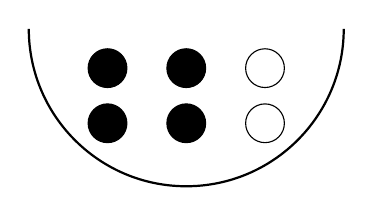
\begin{tikzpicture}
\draw[thick]  (0,0) arc (180:360:2) ;
\filldraw (1,-.5) circle (7pt) (1,-1.2) circle (7pt);
\filldraw (2,-.5) circle (7pt) (2,-1.2) circle (7pt);
\draw (3,-.5) circle (7pt) (3,-1.2) circle (7pt);
\end{tikzpicture}


پیشامد $ E_{1}$ یعنی خارج شدن مهره ی سیاه اول در 3 انتخاب اول 

$$
P(E_{1}) = \frac{\binom{4}{2}\binom{2}{1}}{\binom{6}{3}} = \frac{3}{5}
$$


از طرفی در انتخاب چهارم با احتمال $ \frac{1}{3}$ مهره ی سیاه خارج می شود زیرا از 3 مهره ی باقی مانده فقط یکی سیاه می باید بنابراین :


\begin{tikzpicture}
\draw[thick]  (0,0) arc (180:360:2) ;
\filldraw (1,-1) circle (7pt) ;
\filldraw (2,-1) circle (7pt) ;
\draw (3,-1) circle (7pt) ;
\end{tikzpicture}


$$
P(E_{2}) = \frac{1}{3}
$$

پس داریم :

$$
P(E) = P(E_{1}) \times P(E_{2}) = \frac{3}{5} \times \frac{1}{3} = \frac{3}{15}
$$


\subsubsection{مثال}
جعبه ای حاوی 18 عدد لامپ می باشد، که 6 تای آنها معیوب می باشند، از این جعبه 4 لامپ به تصادف و بدون جایگذاری خارج می کنیم .

\begin{tikzpicture}[level distance=1.3cm,
   level 1/.style={sibling distance=3cm, level distance=1cm},
   level 2/.style={sibling distance=1.5cm, level distance=0.8cm}]
\node {18}
   child {node {6}}
	child {node {12}
};
\end{tikzpicture}


الف ) احتمال اینکه 1 لامپ معیوب در بین اینها باشد چقدر است .

$$
P(E) = \frac{n(E)}{n(S)} = \frac{\binom{6}{1}\binom{12}{3}}{\binom{18}{4}}
$$

ب ) حداقل یک لامپ معیوب باشد .

$$
P(E) = \frac{n(E)}{n(S)} = \frac{
\binom{6}{1}\binom{12}{3} + 
\binom{6}{2}\binom{12}{2} + 
\binom{6}{3}\binom{12}{1} + 
\binom{6}{4}}{\binom{18}{4}}
$$


ج ) حداکثر یک لامپ معیوب باشد .

$$
P(E) = \frac{n(E)}{n(S)} = \frac{
\binom{12}{4} + 
\binom{6}{1}\binom{12}{3}}{\binom{18}{4}}
$$


\subsection{انواع آزمایش تصادفی}


انواع آزمایش تصادفی
\begin{itemize}
	\item کمیت گسسته باشد
		\begin{itemize}
			\item فضای نمونه گسسته
			\begin{itemize}
				\item احتمال گسسته
			\end{itemize}
		\end{itemize}
	\item کمیت پیوسته باشد
		\begin{itemize}
			\item فضای نمونه پیوسته
			\begin{itemize}
				\item احتمال پیوسته
			\end{itemize}
		\end{itemize}
\end{itemize}




نکته : اگر فضای نمونه ناحیه ای از یک طول، مساحت، حجم، زمان و . . . باشد و بخواهیم به تصادف زیرناحیه ای از آن را انتخاب کنیم از رابطه ی زیر استفاده می کنیم 

$$
P(A) = \frac{A(E)}{A(S)}
$$


A به معنی مساحت می باشد 


\subsubsection{مثال}
نقطه ای را به تصادف از داخل مربع به ضلع 2 انتخاب می کنیم، احتمال اینکه فاصله ی آن نقطه از راس های مربع بیشتر از 1 باشد چقدر است ؟



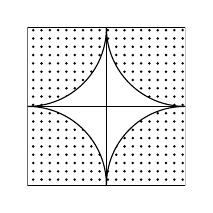
\begin{tikzpicture}
%\draw (-1.5,0) -- (1.5,0);
%\draw (0,-1.5) -- (0,1.5);
\clip (-1,-1) rectangle (1,1);
\draw (-1,-1) rectangle (1,1);
\draw[pattern=dots] (-1,-1) circle (1cm);
\draw[pattern=dots] (1,-1) circle (1cm);
\draw[pattern=dots] (-1,1) circle (1cm);
\draw[pattern=dots] (1,1) circle (1cm);
\draw[step=1cm] (-1.5,-1.5) grid (1.5,1.5);
\end{tikzpicture}

\begin{align*}
A(S) &= 2 \times 2 = 4 \\
A(E') &= \pi r^{2} = \pi (1)^{2} = \pi \\
A(E) &= 4 - \pi \\
\end{align*}

$$
P(E) = \frac{A(E)}{A(S)} = \frac{4-\pi}{4} = 1 - \frac{\pi}{4}
$$


\subsubsection{مثال}
نقطه ای را به تصادف روی سطح دایره ای انتخاب می کنیم، احتمال اینکه فاصله ی نقطه ی انتخابی از مرکز دایره کمتر از فاصله ی آن نقطه تا محیط دایره باشد چقدر است ؟

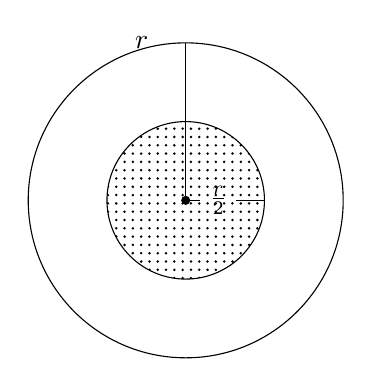
\begin{tikzpicture}
\draw (0,0) -- (0,2) node[below=10pt,left=10pt,fill=white] {$r$};
\draw (0,0) -- (1,0) node[below=2pt,left=10pt,fill=white] {$\frac{r}{2}$};
\draw (0,0) circle (2cm);
\draw[pattern=dots] (0,0) circle (1cm);
\filldraw[color=black] (0,0) circle (.05cm);
\end{tikzpicture}

\begin{align*}
A(S) &= \pi r^{2} \\
A(E) &= \pi (\frac{r}{2})^{2} = \pi \frac{r^{2}}{4} \\
\end{align*}


$$
P(E) = \frac{A(E)}{A(S)} = \frac{\pi \frac{r^{2}}{4}}{\pi r^{2}} = \frac{1}{4}
$$


در صورتی که نقطه ی انتخابی از مرکز دایره بیشتر از فاصله ی نقطه تا محیط دایره باشد چقدر است :

\begin{align*}
A(S) &= \pi r^{2} - \pi \frac{r^{2}}{4} = \frac{3 \pi r^{2}}{4} \\
\end{align*}

$$
P(E) = \frac{A(E)}{A(S)} = \frac{3 \pi \frac{r^{2}}{4}}{\pi r^{2}} = \frac{3}{4}
$$


\subsubsection{مثال}
یک نقطه به تصادف از این محدوده انتخاب می شود

$$
\{ (x, y) | 0 < x < 2 , 0 < y < 2 \}
$$

احتمال اینکه 
$$
x^{2} + y^{2} < 4
$$

برقرار باشد چقدر است ؟

\begin{tikzpicture}
\clip (0,0) rectangle (4,4);
\draw (-1.5,0) -- (1.5,0);
\draw (0,-1.5) -- (0,1.5);
\draw (1,-2) -- (1,2) node[above=10pt]{$x=2$};
\draw (-2,1) -- (2,1) node[right=10pt]{$y=2$};
\draw[pattern=dots] (0,0) circle (1cm);
\draw[step=1cm] (-1.5,-1.5) grid (1.5,1.5);
\end{tikzpicture}


\begin{align*}
A(S) &= 2 \times 2  = 4 \\
A(E) &= \pi \frac{r^{2}}{4} = \frac{\pi (2^{2})}{4} = \frac{4\pi}{4} = \pi 
\end{align*}


$$
P(E) = \frac{A(E)}{A(S)} = \frac{\pi}{4}
$$

\subsection{قضایای احتمال}

1 ) 

$$
P(E) = 1 - P(E')
$$

اثبات : هر پیشامد یک مجموعه است بنابراین تمام قواعد مجموعه ها بر پیشامدها نیز برقرار است .

نتیجه : 
$$
P(E) + P(E') = 1
$$

2 ) طبق اصول سه گانه ی احتمال :

\begin{align*}
P(S) &= 1 \\
P(S) &= \Rightarrow P(\phi) = 0 \\ 
\end{align*}

اثبات ( برای دوم ) :
$$
S' = \phi
$$

$$
P(\phi) = 1 - P(S) = 1 - 1 = 0
$$


\subsubsection{مثال}

یک سکه را حداقل چند بار پرتاب کنیم تا احتمال آمدن حداقل یک شیر بیش از 99 درصد باشد ؟

برای پرتاب یکبار تاس داریم :
$$
S = \{ H , T \}
$$

برای پرتاب 2 بار تاس، احتمال حداقل یک شیر برابر است با :

$$
S = \{ HH , HT, TH, TT \}  \Rightarrow P( H \geq 1 ) = 1 -(\frac{1}{2})^{2}
$$

برای پرتاب 3 بار تاس، احتمال حداقل یک شیر برابر است با :


$$
S = \{ HHH , HHT, HTH, THH, HTT, THT, TTH, TTT \}  \Rightarrow P( H \geq 1 ) = 1 -(\frac{1}{2})^{3}
$$


\begin{align*}
&\Rightarrow \\
1 - (\frac{1}{2})^{n} &> \frac{99}{100} \\
1 - \frac{99}{100} &> (\frac{1}{2})^{n} \\
\frac{1}{100} &> \frac{1}{2^{n}} \\
100 &< 2^{n} \\
2^{n} &> 100 \\
\ln{2^{n}} &> \ln{100} \\
n \ln{2} &> \ln{100} \\
n \frac{ \ln{2}}{ \ln{2}} &> \frac{ \ln{100}}{ \ln{2}} \\
n &> \ln{50} \\
&\simeq 7
\end{align*}

بنابراین از پرتاب هفتم به بعد به احتمال 99 درصد حداقل یکبار شیر می آید .

\newpage

\subsubsection{مثال}
یک خانواده چند فرزند داشته باشد تا با احتمال 95 درصد یک پسر و یک دختر داشته باشد ؟

\newpage


\subsection{احتمال شرطی}

در بسیاری از مسائل می خواهیم احتمال وقوع یک پیشامد با این فرض که پیشامد دیگری به وقوع پیوسته است . به عبارت دیگر :

اگر احتمال پیشامدی مانند E را مشروط بر معلوم بودن پیشامد دیگری مانند F بدانیم ، این نوع احتمال ها را احتمال های شرطی می دانیم .

$$
P( E | F ) = \frac{P( E \cap F )}{P(F)} 
$$


\subsubsection{مثال}
2 تاس سالم را با هم پرتاب می کنیم، اگر بدانیم شماره ی روی تاس اول 3 باشد ( F ) ، احتمال اینکه مجموع ارقام روی 2 تاس برابر 8 باشد ( E ) را پیدا کنید ؟

$$
P( E | F ) =  \frac{P( E \cap F )}{P(F)} 
$$

E $\leftarrow$ مجموع ارقام روی 2 تاس 8 باشد

F $\leftarrow$ شماره ی روی تاس اول 3 باشد

\begin{align*}
E &= \{ ( 2, 6 ), ( 6, 2 ), ( 3, 5 ), ( 5, 3 ), ( 4, 4 ) \} \\
F &= \{ ( 3, 1 ), ( 3, 2 ), ( 3, 3 ), ( 3, 4 ), ( 3, 5 ), ( 3, 6 ) \} \\
E \cap F &= \{ ( 3, 5 ) \}
\end{align*}

برای پرتاب 2 تاس داریم :
$$
n(S) = 36
$$

$$
P( E | F ) =  \frac{P( E \cap F )}{P(F)}  = \frac{\frac{1}{36}}{\frac{6}{36}}  = \frac{1}{6}
$$


\subsubsection{مثال}
عددی را به تصادف از بین اعداد طبیعی 1 تا 100 انتخاب می کنیم، اگر بدانیم که عدد انتخاب شده زوج باشد ( F ) ، احتمال اینکه بر پنج بخش پذیر نباشد ( E ) ، چقدر است ؟


$n(S) = 100$ $\leftarrow$ انتخاب یک عدد بین 1 تا 100

$n(F) = 50$ $\leftarrow$ تعداد اعداد زوج بین 1 تا 100

$n(E') = 10$ $\leftarrow$ تعداد اعداد بخش پذیر بر 5 که زوج باشد

$$
n ( F \cap E ) = n ( F - E' ) = 50 - 10 = 40
$$


$$
P( E | F ) =  \frac{P( E \cap F )}{P(F)}  = \frac{\frac{40}{100}}{\frac{50}{100}}  = \frac{4}{5}
$$


نکته :

$$
A \cap B = A - B'
$$



\subsection{متغیرهای تصادفی}
در مطالب قبل پیشامدهای مربوط به یک آزمایش تصادفی به صورت تصادفی مورد مطالعه قرار گرفته اند .

در این فصل می خواهیم با تعریف تابعی از فضای نمونه به مجموعه اعداد حقیقی، بیان توصیفی را به بیان عددی تبدیل می کنیم .

چنین توابعی متغیرهای تصادفی نامیده می شوند .
$$
f : S \to {\Bbb R}
$$


\subsubsection{مثال}
آزمایش پرتاب 2 تاس را در نظر بگیرید و متغیر تصادفی روی فضای نمونه همان مجموع شماره های ظاهر شده بر روی 2 تاس باشد، در این صورت حاصل متغیر تصادفی را به دست آورید ؟

$$
S = \{ ( i , j ) | i , j \in [ 1 , 6 ] \}
$$


بنابراین برای $S_{x}$ که مجموع شماره های روی تاس باشد داریم :

$$
S_{x} = \{ \underbrace{2}_{1+1} , \underbrace{3}_{1+2 , 2+1} , \underbrace{4}_{1+3 , 3+1 , 2+2} , 5 , 6 , 7 , 8 , 9 , 10 , 11 , 12 \} 
$$

\subsubsection{مثال}
می توان مثال قبل را به صورت تفاضل شماره های روی 2 تاس برای متغیر تصادفی در نظر گرفت ؟

$$
X = | i - j | \to S_{x} = \{ 0 , 1 , 2 , 3 , 4 , 5 \}
$$



\subsubsection{مثال}
آزمایش پرتاب 2 سکه را در نظر بگیرید و متغیر تصادفی تعریف شده روی فضای نمونه تعداد شیرهایی باشد که ظاهر می شود ؟

\begin{align*}
S &= \{ HH, TH, HT, TT \} \\
S_{x} &= \{ \underbrace{0}_{TT} , \underbrace{1}_{TH , HT}, \underbrace{2}_{HH} \}
\end{align*}


\subsubsection{نکته}

اصول شمارش $\leftarrow$ احتمال   $\leftarrow$  احتمال شرطی  $\leftarrow$  متغیر تصادفی 



\subsubsection{نکته}

مطالبی که در قسمت قبل گفته شد مربوط به متغیرهای تصادفی می باشد، حال فرض کنید که $x \in S_{x}$ در این صورت خواهیم داشت ، 
$$
X : S \to R \Rightarrow X^{-1} : R \to S
$$

چون ما همه ی اعداد حقیقی را به وجود نمی آوریم بلکه زیر مجموعه ای از اعداد حقیقی را به وجود می آوریم بنابراین به جای R می نویسیم $S_{x}$ :

$$
X^{-1} : S_{x} \to S
$$

$$
X^{-1}(x) = \{ s \in S ; X(s) = x \}
$$


برای مثال برای پرتاب 2 سکه داریم :

متغیر تصادفی $\leftarrow$ تعداد شیر های ظاهر شده

\begin{align*}
S_{x} &= \{ 0 , 1 , 2 \} \\
X^{-1}(0) &= \{ TT \} \\
X^{-1}(1) &= \{ TH, HT \} \\
X^{-1}(2) &= \{ HH \} \\
\end{align*} 


\subsubsection{نکته}

از آنجایی که عکس متغیر تصادفی یک پیشامد می باشد، لذا احتمال آن قابل محاسبه است و می توان به این فرم نشان داد :

$$
P ( X^{-1} ) = f_{X}(x)
$$

که به آن توزیع احتمال متغیر تصادفی یا تابع احتمال متغیر تصادفی می نامیم .

متغیر تصادفی  $\leftarrow$  عکس متغیر تصادفی   $\leftarrow$   احتمال عکس متغیر تصادفی   

\subsubsection{نکته}
توزیع احتمال روی پیشامد عکس متغیر تصادفی اثر می کند .


\subsubsection{تعریف}
اگر X یک متغیر تصادفی باشد ( گسسته ) ، تابع احتمال یا توزیع احتمال در 2 شرط زیر صدق می کند .


\begin{enumerate}
	\item $0 \leq f(x) \leq 1$
	\begin{itemize}
		\item موقعی
		$f_{X}(x) = 0$
		می شود که پیشامد تهی باشد یا عضوی نداشته باشد
		\item موقعی
		$f_{X}(x) = 1$
		می شود که پیشامد شامل تمام عضوهای فضای نمونه باشد 
	\end{itemize}
	\item $$\sum_{x \in S_{x}}{f_{X}(x)} = 1$$
\end{enumerate}




\subsubsection{مثال}
بررسی کنید که تابع


$$
f_{X}(x) = 
\begin{cases}
\frac{2(n-x)+1}{n^{2}} & x=1,2,3,\dots,n \\
0 & other.wise
\end{cases}
$$

تابع احتمال هست یا نه ؟


الف ) به آسانی می توان نشان داد که
$f_{X}(x)$
نامنفی می باشد .

\begin{align*}
n^{2} &> 0 \\
x &\leq n \\
n &\geq x \\
n - x &\geq 0 \\
f_{X}(x) &\geq 0 \\
\end{align*}


ب ) برای شرط دوم $\sum_{x \in S_{x}} f_{X}(x) = 1$

\begin{align*}
&\sum_{x=1}^{n}{(\frac{2(n-x)+1}{n^{2}})} \\
&= \sum_{x=1}^{n}{(\frac{2(n-x)}{n^{2}})} + \sum_{x=1}^{n}{(\frac{1}{n^{2}})} \\
&= \frac{2}{n^{2}}  \sum_{x=1}^{n}{(n-x)} + \frac{1}{n^{2}}  \sum_{x=1}^{n}{(1)}  \\
&= \frac{2}{n^{2}} ( (n-1) + (n-2) + \dots + 1 + 0 ) +
\frac{1}{n^{2}} ( \underbrace{1 + 1 + 1 + \dots + 1}_{n \:\: times} ) \\
&= \frac{2}{n^{2}} (\frac{n( ( n - 1 ) + 0 )}{2}) + \frac{1}{n^{2}} ( n ) \\
&= \frac{n( n - 1 )}{n^{2}} + \frac{n}{n^{2}} \\
&= \frac{ n - 1 }{n} + \frac{1}{n} \\
&= \frac{ n - 1 + 1 }{n} \\
&= \frac{ n }{n}  \\
&= 1 \\
\end{align*}


بنابراین مجموع جملات توزیع احتمال برابر 1 است 

\subsubsection{نکته}
مجموع جملات تصاعد حسابی

$$
S_{n} = \frac{n(a_{1} + a_{n})}{2}
$$



\subsubsection{مثال}
جعبه ای شامل 4 مهره به شماره های 1 و 2 و 3 و 4 می باشد ، 2 مهره به تصادف و بدون جایگذاری از جعبه خارج می کنیم.

متغیر تصادفی X شماره ی بزرگتر بر روی 2 مهره ی انتخابی را تعریف می کند، تابع احتمال این متغیر تصادفی را محاسبه کنید .

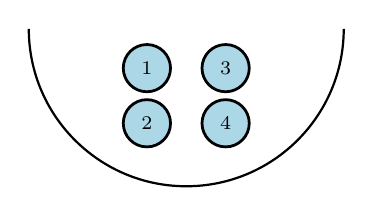
\begin{tikzpicture}
\draw[thick]  (0,0) arc (180:360:2) ;
\Vertex[x=1.5,y=-.5,label=$1$]{A1}
\Vertex[x=1.5,y=-1.2,label=$2$]{A2}

\Vertex[x=2.5,y=-.5,label=$3$]{B1}
\Vertex[x=2.5,y=-1.2,label=$4$]{B2}
\end{tikzpicture}


تعداد اعضای فضای نمونه برابر است با :

$$
n(S) = \binom{4}{2} = \frac{4!}{2!2!} = \frac{4 \times 3 \times 2!}{2! \times 2} = 6
$$


فضای نمونه :

$$
S = \{ ( 1 , 2 ), ( 1 , 3 ), ( 1 , 4 ), ( 2 , 3 ), ( 2 , 4 ), ( 3 , 4 ) \}
$$


متغیر تصادفی X ( شماره ی بزرگتر ) :

$$
S_{X} = \{ 2 , 3 , 4 \}
$$


\begin{align*}
X^{-1}(2) &= \{  ( 1 , 2 ) \} \\
X^{-1}(3) &= \{  ( 1 , 3 ),  ( 2 , 3 ) \} \\
X^{-1}(4) &= \{  ( 1 , 4 ), ( 2 , 4 ), ( 3 , 4 ) \} \\
\end{align*}


نکته : چون عکس متغیر تصادفی یک زیر مجموعه از فضای نمونه است ، بنابراین پیشامد است به این دلیل می توان برای آن تابع احتمال تعریف کرد .

تعریف ریاضی عکس متغیر تصادفی :
$$
X^{-1}(x) = \{ s \in S | X(s) = x \}
$$


\begin{align*}
P(X^{-1}(2)) &= f_{X}(2) = \frac{1}{6} \\
P(X^{-1}(3)) &= f_{X}(3) = \frac{2}{6} \\
P(X^{-1}(4)) &= f_{X}(4) = \frac{3}{6} \\
\end{align*}

جدول تابع احتمال :

\begin{center}
\begin{latin}
\begin{tabular}{ l |  l  l  l  }
  $x$ & 2 & 3 & 4  \\
  \hline
  $f_{X}(x)$ & $\frac{1}{6}$ & $\frac{2}{6}$ & $\frac{3}{6}$  \\
\end{tabular}
\end{latin}
\end{center}


\subsubsection{مثال}

سکه ای را احتمال آمدن شیر در آن سه برابر خط می باشد را سه مرتبه پرتاب می کنیم، متغیر تصادفی تعداد شیرهای ظاهر شده تعریف می شود .

الف ) توزیع احتمال این متغیر تصادفی را به دست آورید

ب ) احتمال 
$P(1 \leq X < 3)$
و 
$P(x \geq 1)$
را به دست آورید .

جواب : 

تعداد اعضای فضای نمونه برابر است با :

$$
2 \times 2 \times 2 = 2^{3} = 8
$$

$$
S = \{ HHH , HHT, HTH, THH, HTT, THT, TTH , TTT \}
$$

متغیر تصادفی ( X ) برابر با تعداد شیرهای ظاهر شده است، بنابراین داریم :

\begin{align*}
S_{X} &= \{ 0, 1, 2, 3 \} \\
X^{-1}(0) &= \{ TTT \} \\
X^{-1}(2) &= \{ HTT, THT, TTH \} \\
X^{-1}(3) &= \{ HHT, HTH, THH \} \\
X^{-1}(4) &= \{ HHH \} \\
\end{align*}


\begin{align*}
P(X^{-1}(0)) &= f_{X}(0) = \frac{1}{64} & \{ TTT \}  \\
P(X^{-1}(1)) &= f_{X}(1) = \frac{9}{64} &  \{ HTT, THT, TTH \} \\
P(X^{-1}(2)) &= f_{X}(2) = \frac{27}{64} & \{ HHT, HTH, THH \} \\
P(X^{-1}(3)) &= f_{X}(3) = \frac{27}{64} & \{ HHH \} \\
\end{align*}



\begin{center}
\begin{latin}
\begin{tabular}{ l |  l  l  l  l }
  $x$ & 0 & 1 & 2 & 3  \\
  \hline
  $f_{X}(x)$ & $\frac{1}{64}$ & $\frac{9}{64}$ & $\frac{27}{64}$  & $\frac{27}{64}$ \\
\end{tabular}
\end{latin}
\end{center}



بنابراین برای محاسبه ی 
$P(1 \leq X < 3)$
و
$P(x \geq 1)$
داریم :

\begin{align*}
P(1 \leq X < 3) &= P( X = 1 ) + P( X = 2 ) \\
&= \frac{9}{64} + \frac{27}{64} = \frac{36}{64} 
\end{align*}


\begin{align*}
P(X \geq 1) &= P( X = 1 ) + P( X = 2 ) + P( X = 3 ) \\
&= \frac{9}{64} + \frac{27}{64}+ \frac{27}{64} \\
&= \frac{63}{64} 
\end{align*}



\subsubsection{مثال}

متغیر تصادفی X دارای توزیع احتمال 
$$
f_{X}(x) = k (\frac{2}{3})^{x} ; \qquad x = 0 ,1 , 2, \dots
$$

الف ) مقدار ثابت k را به دست آورید .

ب ) توزیع احتمال 
$P( X \geq 2 )$
و
$P( 2 \leq X < 5 )$
را به دست آورید .

جواب : از آنجایی که تابع f دارای خاصیت های تابع احتمال می باشد، لذا می توان نوشت .

1 :

$$
f_{X}(x) \geq 0
$$

$$
\underbrace{f_{X}(x)}_{positive} = k \underbrace{(\frac{2}{3})^{x}}_{positive} \Rightarrow k > 0
$$


2 :

\begin{align*}
&\sum_{x=0}^{\infty}{k (\frac{2}{3})^{x} } = 1 \\
& k \sum_{x=0}^{\infty}{(\frac{2}{3})^{x} } = 1 \\
& k [1 + \frac{2}{3} + (\frac{2}{3})^{2} + (\frac{2}{3})^{3} + \dots ] = 1 \\
\end{align*}


نکته : مجموع جملات نامتناهی تصاعد هندسی 
$$
S_{\infty} = \frac{a}{1-q}
$$


\begin{align*}
&\Rightarrow \\
&k \times \frac{1}{1 - \frac{2}{3} } = 1 \\
&3 k = 1 \\
&\Rightarrow f_{X}(x) = \frac{1}{3}(\frac{2}{3})^{x} \\
\end{align*}


ب ) 

\begin{center}
\begin{latin}
\begin{tabular}{ l |  l  l  l  l  l }
  $x$ & 0 & 1 & 2 & 3  & 4 \\
  \hline
  $f_{X}(x)$ & $\frac{1}{3}$ & $\frac{2}{9}$ & $\frac{4}{27}$  & $\frac{8}{3^{4}}$ & $\frac{16}{3^{5}}$ \\
\end{tabular}
\end{latin}
\end{center}


\begin{align*}
P(X \geq 2) &= P( X = 2 ) + P( X = 3 ) + P( X = 4 ) + \dots \\
&= \frac{4}{27} + \frac{8}{3^{4}} + \frac{16}{3^{5}}  + \dots
\end{align*}

\begin{align*}
a &= \frac{4}{27} \\
q &= \frac{2}{3} \\
S &= \frac{a}{1-q} \\
&= \frac{\frac{4}{27}}{1-\frac{2}{3}}
\end{align*}

\begin{align*}
P( 2 \leq X < 5 ) &= P( X = 2 ) + P( X = 3 ) + P( X = 4 ) \\
&= \frac{4}{27} + \frac{8}{3^{4}} + \frac{16}{3^{5}} 
\end{align*}



\subsection{امید ریاضی}
فرض کنید یک هدف تیر اندازی داریم که به شکل دایره می باشد، با رسم شعاع هایی به 6 قسمت مساوی تقسیم می کنیم و به ترتیب به آنها  شماره هایی ار 1 تا 6 نسبت دادیم .

تیراندازی که صفحه ی هدف را مورد اصابت قرار می دهد، هر یک از 6 قسمت را با احتمال هایی برابر 
$\frac{1}{6}$
مورد اصابت قرار می دهد . اگر به تیرانداز جایزه ای 10 برابر شماره ی قسمت مورد اصابت پرداخت شود، چه ورودی باید برای هر تیرانداز تعیین شود تا بتوان از محل این ورودی ها جایزه ی تیراندازهای مختلف که وارد بازی می شوند پرداخت نمود .



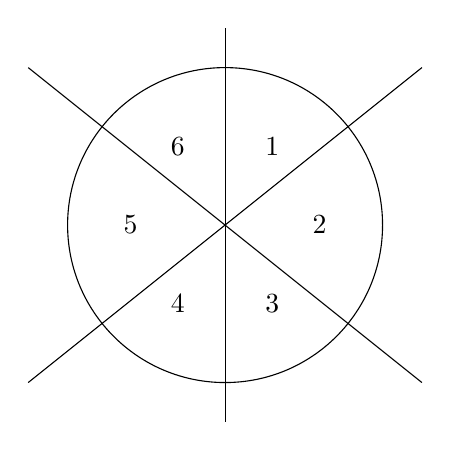
\begin{tikzpicture}
\draw (.6,1) node {1};
\draw (-.6,1) node {6};
\draw (.6,-1) node {3};
\draw (-.6,-1) node {4};
\draw (1.2,0) node {2};
\draw (-1.2,0) node {5};
\draw (0,-2.5) -- (0,2.5);
\draw (-2.5,-2) -- (2.5,2);
\draw (-2.5,2) -- (2.5,-2);
\draw (0,0) circle (2cm);
%\draw[step=.5cm] (-1.4,-1.4) grid (1.4,1.4);
\end{tikzpicture}



$$
S =  \{ 1, 2, 3, 4, 5, 6 \} 
$$

$$
S_{X} = \{ 10, 20, 30, 40, 50, 60 \} 
$$


\begin{align*}
X^{-1}(10) &= \{ 1 \} \\
X^{-1}(20) &= \{ 2 \} \\
X^{-1}(30) &= \{ 3 \} \\
X^{-1}(40) &= \{ 4 \} \\
X^{-1}(50) &= \{ 5 \} \\
X^{-1}(60) &= \{ 6 \} \\
\end{align*}


\begin{align*}
P(X^{-1}(10)) &= f_{X}(10) = \frac{1}{6} \\
P(X^{-1}(20)) &= f_{X}(20) = \frac{1}{6} \\
P(X^{-1}(30)) &= f_{X}(30) = \frac{1}{6} \\
P(X^{-1}(40)) &= f_{X}(40) = \frac{1}{6} \\
P(X^{-1}(50)) &= f_{X}(50) = \frac{1}{6} \\
P(X^{-1}(60)) &= f_{X}(60) = \frac{1}{6} \\
\end{align*}



\begin{center}
\begin{latin}
\begin{tabular}{ l |  l  l  l  l  l  l }
  $x$ & 10 & 20 & 30 & 40  & 50 & 60 \\
  \hline
  $f_{X}(x)$ & $\frac{1}{6}$ & $\frac{1}{6}$ & $\frac{1}{6}$  & $\frac{1}{6}$ & $\frac{1}{6}$ & $\frac{1}{6}$ \\
\end{tabular}
\end{latin}
\end{center}


امید ریاضی برابر است با :

\begin{align*}
E(x) &= 10 \times \frac{1}{6} \\
&+ 20 \times \frac{1}{6} \\
&+ 30 \times \frac{1}{6} \\
&+ 40 \times \frac{1}{6} \\
&+ 50 \times \frac{1}{6} \\
&+ 60 \times \frac{1}{6} \\
\end{align*}


نکته : امید ریاضی برابر است با 

$$
E(x) = \sum_{x}{xf_{X}(x)}
$$


\subsubsection{مثال}
شخصی در یک بازی دو سکه سالم را پرتاب می کند و به اندازه ی تعداد شیرهایی که ظاهر می شود 100 تومان جایزه می برد، چه مبلغی باید بپردازد تا بازی منصفانه شود ؟

\begin{align*}
S &= \{ HH, HT, TH, TT \} \\
S_{X} &= \{ 0, 100, 200 \} \\
X^{-1}(0) &= \{ TT \} \\
X^{-1}(100) &= \{ HT, TH \} \\
X^{-1}(200) &= \{ HH \} \\
P(X^{-1}(0)) &= f_{X}(0) = \frac{1}{4} \\
P(X^{-1}(100)) &= f_{X}(100) = \frac{2}{4} \\
P(X^{-1}(200)) &= f_{X}(200) = \frac{1}{4} \\
\end{align*}


\begin{center}
\begin{latin}
\begin{tabular}{ l |  l  l  l }
  $x$ & 0 & 100 & 200  \\
  \hline
  $f_{X}(x)$ & $\frac{1}{4}$ & $\frac{2}{4}$ & $\frac{1}{4}$   \\
\end{tabular}
\end{latin}
\end{center}



امید ریاضی برابر است با :

\begin{align*}
E(x) &= 0 \times \frac{1}{4} 
+ 100 \times \frac{2}{4} 
+ 200 \times \frac{1}{4} \\
&= \frac{200}{4} + \frac{200}{4} \\
&= \frac{400}{4} \\
&= 100 \\
\end{align*}

بنابراین حداقل مبلغ دریافتی برای بازی منصفانه 100 تومان می باشد .



\subsubsection{مثال}
ضبط صوتی دارای 6 ترانزیستور است که 2 تای آنها معیوب است، فرض کنید 2 تا از این ترانزیستورها را به تصادف انتخاب و از ضبط صوت برداشته و بررسی کنید . 

متغیر تصادفی X تعداد ترانزیستورهای معیوبی باشد که مشاهده می کنیم ، امید ریاضی این متغیر تصادفی را به دست آورید ؟

نکته : در صورتی که بخواهیم اعضای فضای نمونه و اعضای عکس متغیر تصادفی را بنویسیم باید ترانزیستورها را شماره گذاری کنیم .

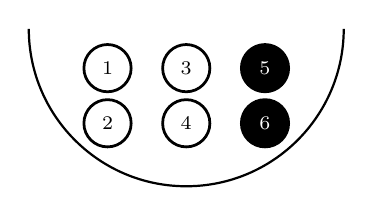
\begin{tikzpicture}
\draw[thick]  (0,0) arc (180:360:2) ;
\Vertex[x=1,y=-.5,label=$1$,color=white,fontcolor=black]{A1}
\Vertex[x=1,y=-1.2,label=$2$,color=white,fontcolor=black]{A2}

\Vertex[x=2,y=-.5,label=$3$,color=white,fontcolor=black]{B1}
\Vertex[x=2,y=-1.2,label=$4$,color=white,fontcolor=black]{B2}

\Vertex[x=3,y=-.5,label=$5$,color=black,fontcolor=white]{C1}
\Vertex[x=3,y=-1.2,label=$6$,color=black,fontcolor=white]{C2}
\end{tikzpicture}


\begin{align*}
S_{X} = \{ 12, 13, 14, 15, 16,& \\
 23, 24, 25, 26,& \\
 34, 35, 36,& \\ 
 45 , 46,& \\ 
 56& \} \Rightarrow n(S) = 15 \\
X^{-1}(0) = \{ 12, 13, 14& \\
 23, 24& \\
 34& \}  \\
X^{-1}(1) = \{ 15, 16,& \\
 25, 26,& \\
 35, 36,& \\
 45 , 46& \}  \\
X^{-1}(2) = \{ 56 \}  \\
\end{align*}


$$
n(S) = \binom{6}{2} = \frac{6!}{4!2!} = \frac{6 \times 5}{2} = 15
$$




\begin{align*}
S_{X} &= \{ 0, 1, 2 \} \\
P(X^{-1}(0)) &= f_{X}(0) = \frac{\binom{4}{2}}{\binom{6}{2}}  = \frac{6}{15} \\
P(X^{-1}(1)) &= f_{X}(1) = \frac{\binom{4}{1}\binom{2}{1}}{\binom{6}{2}} = \frac{8}{15} \\
P(X^{-1}(2)) &= f_{X}(2) = \frac{\binom{2}{2}}{\binom{6}{2}} = \frac{1}{15} \\
\end{align*}




\begin{center}
\begin{latin}
\begin{tabular}{ l |  l  l  l }
  $x$ & 0 & 1 & 2  \\
  \hline
  $f_{X}(x)$ & $\frac{6}{15}$ & $\frac{8}{15}$ & $\frac{1}{15}$   \\
\end{tabular}
\end{latin}
\end{center}





\begin{align*}
E(x) &= 0 \times \frac{6}{15} 
+ 1 \times \frac{8}{15} 
+ 2 \times \frac{1}{15}  \\
&= \frac{8}{15} + \times \frac{2}{15} \\
&= \frac{10}{15} \\
&= \frac{2}{3} \\
\end{align*}


نکته : تابع احتمال برای متغیر تصادفی انتخاب ترانزیستور ها تابع قاعده ی زیر می باشد .

$$
f_{X}(x) = \frac{\binom{2}{x} \binom{4}{2-x}}{\binom{6}{2}} ; \qquad x = 0 , 1 , 2 
$$


\section{توزیع متغیر تصادفی ( گسسته )}

\subsection{توزیع یکنواخت ( $S_{X}$ )}

* اگر حاصل متغیر تصادفی احتمال های برابر داشته باشد .
اگر متغیر تصادفی X مقادیر 
$$
x_{1}, x_{2}, x_{3} , \dots , x_{n}
$$
را با احتمال های یکسان بپذیرد، توزیع احتمال این متغیر تصادفی را یکنواخت می نامیم و پارامتر این توزیع n می باشد .

$$
X \to \{ x_{1}, x_{2}, x_{3} , \dots , x_{n} \}
$$

به آسانی می توان تابع احتمال و امید ریاضی ( میانگین ) و واریانس متغیر تصادفی X را به دست آورید .

$$
\begin{cases}
f_{X}(x) = \frac{1}{n} \\
E(x) = \frac{n+1}{2} \\
var(x) = \frac{n^{2}-1}{12}
\end{cases}
$$



\subsubsection{مثال}
از 10 کارت به شماره های 1 تا 10 کارتی را به تصادف و با جایگذاری ( با تکرار ) انتخاب می کنیم ، متغیر تصادفی شماره ی روی کارت می باشد ، در این صورت تابع احتمال ، امید ریاضی ( میانگین ) و واریانس این متغیر تصادفی را به دست آورید ؟


* چون با جایگذاری انتخاب میکنیم، احتمال ها برابر و بنابراین توزیع یکنواخت می باشد .

حل : چون احتمال انتخاب هر یک از کارت ها یکسان است، بنابراین متغیر تصادفی که همان شماره ی روی کارت می باشد، دارای توزیع یکنواخت می باشد . در این صورت تابع احتمال متغیر تصادفی به فرم $f_{X}(x) = \frac{1}{n}$ نوشته می شود که $n$ پارامتر می باشد .

$$
f_{X}(x) = \frac{1}{n} \qquad ; x = 1 , 2 , 3 , \dots , n
$$

در ایم مثال
 $n=10$
  چون حاصل متغیر تصادفی 10 عضو دارد .


\begin{align*}
S &= \{ 1, 2, 3, \dots , 10 \} \\
X &: S \to R \\
S_{X} &= \{ 1, 2, 3, \dots , 10 \} \\
average &\Rightarrow E(x) = \frac{n+1}{2}  \\
var(x) = \frac{n^{2}-1}{12} 
\end{align*}

$
\Rightarrow
$

\begin{align*}
f_{X}(x) &= \frac{1}{n} \xrightarrow{n=10} f_{X}(x) = \frac{1}{10} \\
average \Rightarrow E(x) &= \frac{n+1}{2} \xrightarrow{n=10} E(x) = \frac{11}{2}  \\
var(x) &= \frac{n^{2}-1}{12}  \xrightarrow{n=10} var(x) = \frac{99}{12}
\end{align*}



\subsection{توزیع برنولی}
آزمایشی که تنها دارای 2 نتیجه باشد، موفقیت و شکست

به طوریکه وقوع همزمان این نتایج امکان پذیر نباشد .

در این حالت این نوع آزمایش را برنولی می نامیم .

اگر احتمال موفقیت را $p$ بنامیم . در این صورت احتمال شکست
$1-p$
می باشد و آن را با $q$ نشان می دهیم، در این صورت متغیر تصادفی به این فرم تعریف می شود .

$$
X = 
\begin{cases}
1 & success \\
0 & failure\\
\end{cases}
$$

که $X$ را توزیع برنولی با پارامتر P می نامیم .
در این صورت تابع احتمال این متغیر تصادفی برابر است با :
$$
f_{X}(x) = p^{x} q ^{1-x} \qquad ; x = 0 , 1 
$$



\begin{center}
\begin{latin}
\begin{tabular}{ l |  l  l }
  $x$ & 0 & 1 \\
  \hline
  $f_{X}(x)$ & $q$ & $p$ \\
\end{tabular}
\end{latin}
\end{center}

اگر X=0 قرار دهیم، $f_{X}(x)$ احتمال شکست را به ما می دهد

اگر X=1 قرار دهیم، $f_{X}(x)$ احتمال موفقیت را به ما می دهد

فرمول های تابع احتمال، امید ریاضی و واریانس طبق فرمولهای زیر محاسبه می شوند .

$$
\begin{cases}
f_{X}(x) = p^{x} q^{1-x} \\
E(x) = p \\
var(x) = pq \\
\end{cases}
$$


\subsubsection{مثال}
کیسه ای شامل 4 مهره ی سفید و 6 مهره ی سیاه می باشد، مهره ای به تصادف از کیسه انتخاب می کنیم و متغیر تصادفی را به فرم زیر تعریف می کنیم .
$$
X = 
\begin{cases}
1  \qquad black \qquad \to p = \frac{6}{1} \\
0 \qquad white \qquad \to q = \frac{4}{10} \\
\end{cases}
$$


$$
f_{X}(x) = (\frac{6}{10})^{x} (\frac{4}{10})^{1-x}
$$



\begin{center}
\begin{latin}
\begin{tabular}{ l |  l  l }
  $x$ & 0 & 1 \\
  \hline
  $f_{X}(x)$ & $\frac{4}{10}$ & $\frac{6}{10}$ \\
\end{tabular}
\end{latin}
\end{center}




$$
E(x) = p = \frac{6}{10}
$$

$$
var(x) = pq = \frac{4}{10} \times \frac{6}{10}
$$


توضیحات : مهره ی انتخاب شده می تواند سیاه یا سفید باشد، لذا این آزمایش برنولی می باشد، چون احتمال مهره ی سیاه موفقیت می باشد لذا
$$
p = \frac{6}{10}
$$
می باشد .


\subsubsection{مثال}
تاسی که احتمال آمدن هر عدد در آن متناسب با عدد روی هر قسمت آن است . یکبار پرتاب می کنیم . و متغیر تصادفی را به صورت زیر تعریف می کنیم ، 
$$
X = 
\begin{cases}
1 & odd \:\: number \\
0 & even \:\: number \\
\end{cases}
$$


ابتدا مدل احتمال برای این آزمایش را تشکیل می دهیم .


\begin{center}
\begin{latin}
\begin{tabular}{ l | l  l  l  l  l  l }
  $S_{i}$ & 1 & 2 & 3 & 4  & 5 & 6 \\
  \hline
  $P(S_{i})$ & 1x & 2x & 3x & 4x  & 5x & 6x \\
\end{tabular}
\end{latin}
\end{center}

$$
\sum_{i=1}^{6}{P(S_{i})} = 1 \Rightarrow 21 x = 1 \Rightarrow x = \frac{1}{21}
$$



\begin{align*}
S_{odd} &= \{ 1 , 3 , 5 \} \\
S_{even} &= \{ 2 , 4 , 6 \} \\
P(odd) &= P(success) = \frac{1}{21} + \frac{3}{21} + \frac{5}{21} = \frac{9}{21} \\
P(even) &= P(failure) = 1 - \frac{9}{21} = \frac{21}{21} - \frac{9}{21} = \frac{12}{21} \\
\end{align*}


$$
f_{X}(x) = p^{x} q^{1-x} \Rightarrow
$$

\begin{center}
\begin{latin}
\begin{tabular}{ l |  l  l }
  $x$ & 0 & 1 \\
  \hline
  $f_{X}(x)$ & $\frac{12}{21}$ & $\frac{9}{21}$ \\
\end{tabular}
\end{latin}
\end{center}

$$
\begin{cases}
E(x) = p \to E(x) = \frac{9}{21} \\
var(x) = pq \to var(x) = \frac{9}{21} \times \frac{12}{21} \\
\end{cases}
$$



\subsection{توزیع دو جمله ای}
هرگاه آزمایش برنولی با احتمال موفقیت p ، 
n بار به طور مستقل تکرار شود، این آزمایش را دو جمله ای می نامیم .

اگر متغیر تصادفی تعداد موفقیت ها در یک آزمایش دو جمله ای تعریف شود . در این صورت X به عنوان یک متغیر تصادفی دو جمله ای دارای 2 پارامتر می باشد .

$$
X = 
\begin{cases}
n \qquad repetition\\
p \qquad success \:\: probability\\
\end{cases}
$$


لذا می توان تابع احتمال این توزیع را به صورت زیر نوشت .

$$
\begin{cases}
f_{X}(x) = \binom{n}{x} p^{x} q^{n-x} \qquad ; x = 0 , 1 , \dots , n \\
E(x) = np \\
var(x) = npq \\
\end{cases}
$$



\subsubsection{مثال}
20\% قطعات تولید شده در خط تولید کارخانه ای ناسالم است . مهندس کنترل کیفیت این کارخانه در هر شیفت کاری 10 قطعه ی تولید شده را مورد آزمایش قرار می دهد .

( یعنی آزمایش برنولی که 10 بار تکرار شود )

$$\Rightarrow n = 10$$

احتمال اینکه در یک شیفت کاری او 4 قطعه ی ناسالم در این قطعات پیدا کند چقدر است ؟ (
$x=4$
)



P(موفقیت) = $\frac{2}{10}$

P(شکست) = $\frac{8}{10}$

حل : فرض کنیم X متغیر تصادفی تعداد قطعات ناسالم باشد، که در این صورت :

P(قطعات-ناسالم) = $\frac{2}{10}$


q = 1 - P(موفقیت) = 1 - $\frac{2}{10}$ = $\frac{8}{10}$


$$
f_{X}(x) = \binom{10}{x} (\frac{2}{10})^{x} (\frac{8}{10})^{10-x}
$$

$$
x = 4 \Rightarrow f_{X}(4) = \binom{10}{4} (\frac{2}{10})^{4} (\frac{8}{10})^{10-4}
$$

$$
E(x) = np = 10 \times \frac{2}{10} = 2
$$

$$
var(x) = npq = 10 \times \frac{2}{10} \times \frac{8}{10} = \frac{16}{10}
$$


نکته : در این مثال اگر 
$x = 0$
یعنی در آزمایش هیچ قطعه ی ناسالمی پیدا نشود .



\subsubsection{مثال}
احتمال اینکه تیراندازی تیری را به هدف بزند 
$\frac{1}{3}$
است .

اگر تیرانداز 5 بار شلیک کند، 
$(n = 5)$

مطلوب است :

الف ) احتمال اینکه دقیقاً 3 تیر به هدف برخورد کند . 
$(x = 3)$

ب ) حداقل 2 تیر به هدف برخورد کند .

ج ) او چند تیر باید شلیک کند تا با احتمال بیش از 95\% هدف را بزند .

جواب الف )
\begin{align*}
P(success) &= \frac{1}{3} \\
n &= 5 \\
x &= 3 \\
\end{align*}

بنابراین داریم
\begin{align*}
f_{X}(x) &= \binom{n}{x} p^{x} q^{n-x} \\
f_{X}(4) &= \binom{5}{3} (\frac{1}{3})^{3} (\frac{2}{3})^{5-3}
\end{align*}


جواب ب )
\begin{align*}
f_{X}(2 \leq x \leq 5) &= f_{X}(2) + f_{X}(3) + f_{X}(4) + + f_{X}(5) \\
&= \binom{5}{2} (\frac{1}{3})^{2} (\frac{2}{3})^{5-2} + \binom{5}{3} (\frac{1}{3})^{3} (\frac{2}{3})^{5-3} + \binom{5}{4} (\frac{1}{3})^{4} (\frac{2}{3})^{5-4} + \binom{5}{5} (\frac{1}{3})^{5} (\frac{2}{3})^{5-5}
\end{align*}

جواب ج )


P(هیچ-تیری-به-هدف-برخورد-نکند) - 1
= P(تیری-به-هدف-برخورد-کند) 

\begin{align*}
= 1 - P(X=0) &\geq 0.95 \\
\Rightarrow 1 - \binom{n}{0} (\frac{1}{3})^{0} (\frac{2}{3})^{n-0} &\geq 0.95 \\
\Rightarrow  1 - (\frac{2}{3})^{n} &\geq 0.95 \\
\Rightarrow 1 - \frac{95}{100} &\geq (\frac{2}{3})^{n} \\
\Rightarrow \frac{5}{100} &\geq  (\frac{2}{3})^{n} \\
\Rightarrow \ln{\frac{5}{100}} &\geq \ln{(\frac{2}{3})^{n}} \\
\Rightarrow \ln{\frac{5}{100}} &\geq n\ln{(\frac{2}{3})} \\
\Rightarrow n &\geq 6
\end{align*}

\end{document}